\documentclass[a4paper, 12pt]{article}
\usepackage[brazil]{babel}
\usepackage{indentfirst}
\usepackage{graphicx}
\usepackage{graphics}

\usepackage{tabularx}
\usepackage{graphicx}
\usepackage{adjustbox}

\usepackage{booktabs}
\usepackage[font=footnotesize,labelfont=bf]{caption} %muda o tamanho das caption e deixa em negrito
\usepackage{cite}
\usepackage{color}   %May be necessary if you want to color links
\usepackage{hyperref}
\hypersetup{
    colorlinks=true,
    citecolor=blue,
    filecolor=blue,
    linkcolor=blue,
    urlcolor=blue
}
%%%%%%%%%%%%%%%%%%%%%%%%%%%%%%%%%%%%%%%%%%%%%%%%
%%%%%%%%%%%%%%%%%%%%JUPYTER TEX%%%%%%%%%%%%%%%%%
%%%%%%%%%%%%%%%%%%%%%%%%%%%%%%%%%%%%%%%%%%%%%%%%
\usepackage[breakable]{tcolorbox}
\tcbset{nobeforeafter} % prevents tcolorboxes being placing in paragraphs
\usepackage{float}
\floatplacement{figure}{H} % forces figures to be placed at the correct location

\usepackage[T1]{fontenc}
% Nicer default font (+ math font) than Computer Modern for most use cases
\usepackage{mathpazo}

% Basic figure setup, for now with no caption control since it's done
% automatically by Pandoc (which extracts ![](path) syntax from Markdown).
\usepackage{graphicx}
% We will generate all images so they have a width \maxwidth. This means
% that they will get their normal width if they fit onto the page, but
% are scaled down if they would overflow the margins.
\makeatletter
\def\maxwidth{\ifdim\Gin@nat@width>\linewidth\linewidth
\else\Gin@nat@width\fi}
\makeatother
\let\Oldincludegraphics\includegraphics
% Set max figure width to be 80% of text width, for now hardcoded.
% \renewcommand{\includegraphics}[1]{\Oldincludegraphics[width=.8\maxwidth]{#1}}
% Ensure that by default, figures have no caption (until we provide a
% proper Figure object with a Caption API and a way to capture that
% in the conversion process - todo).

\usepackage{caption}
\DeclareCaptionLabelFormat{nolabel}{}
\captionsetup{labelformat=nolabel}

\usepackage{adjustbox} % Used to constrain images to a maximum size 
\usepackage{xcolor} % Allow colors to be defined
\usepackage{enumerate} % Needed for markdown enumerations to work
\usepackage{geometry} % Used to adjust the document margins
\usepackage{amsmath} % Equations
\usepackage{amssymb} % Equations
\usepackage{textcomp} % defines textquotesingle
% Hack from http://tex.stackexchange.com/a/47451/13684:
\AtBeginDocument{%
    \def\PYZsq{\textquotesingle}% Upright quotes in Pygmentized code
}
\usepackage{upquote} % Upright quotes for verbatim code
\usepackage{eurosym} % defines \euro
\usepackage[mathletters]{ucs} % Extended unicode (utf-8) support
\usepackage[utf8x]{inputenc} % Allow utf-8 characters in the tex document
\usepackage{fancyvrb} % verbatim replacement that allows latex
\usepackage{grffile} % extends the file name processing of package graphics 
                     % to support a larger range 
% The hyperref package gives us a pdf with properly built
% internal navigation ('pdf bookmarks' for the table of contents,
% internal cross-reference links, web links for URLs, etc.)
\usepackage{hyperref}
\usepackage{longtable} % longtable support required by pandoc >1.10
\usepackage{booktabs}  % table support for pandoc > 1.12.2
\usepackage[inline]{enumitem} % IRkernel/repr support (it uses the enumerate* environment)
\usepackage[normalem]{ulem} % ulem is needed to support strikethroughs (\sout)
                            % normalem makes italics be italics, not underlines
\usepackage{mathrsfs}



% Colors for the hyperref package
\definecolor{urlcolor}{rgb}{0,.145,.698}
\definecolor{linkcolor}{rgb}{.71,0.21,0.01}
\definecolor{citecolor}{rgb}{.12,.54,.11}

% ANSI colors
\definecolor{ansi-black}{HTML}{3E424D}
\definecolor{ansi-black-intense}{HTML}{282C36}
\definecolor{ansi-red}{HTML}{E75C58}
\definecolor{ansi-red-intense}{HTML}{B22B31}
\definecolor{ansi-green}{HTML}{00A250}
\definecolor{ansi-green-intense}{HTML}{007427}
\definecolor{ansi-yellow}{HTML}{DDB62B}
\definecolor{ansi-yellow-intense}{HTML}{B27D12}
\definecolor{ansi-blue}{HTML}{208FFB}
\definecolor{ansi-blue-intense}{HTML}{0065CA}
\definecolor{ansi-magenta}{HTML}{D160C4}
\definecolor{ansi-magenta-intense}{HTML}{A03196}
\definecolor{ansi-cyan}{HTML}{60C6C8}
\definecolor{ansi-cyan-intense}{HTML}{258F8F}
\definecolor{ansi-white}{HTML}{C5C1B4}
\definecolor{ansi-white-intense}{HTML}{A1A6B2}
\definecolor{ansi-default-inverse-fg}{HTML}{FFFFFF}
\definecolor{ansi-default-inverse-bg}{HTML}{000000}

% commands and environments needed by pandoc snippets
% extracted from the output of `pandoc -s`
\providecommand{\tightlist}{%
  \setlength{\itemsep}{0pt}\setlength{\parskip}{0pt}}
\DefineVerbatimEnvironment{Highlighting}{Verbatim}{commandchars=\\\{\}}
% Add ',fontsize=\small' for more characters per line
\newenvironment{Shaded}{}{}
\newcommand{\KeywordTok}[1]{\textcolor[rgb]{0.00,0.44,0.13}{\textbf{{#1}}}}
\newcommand{\DataTypeTok}[1]{\textcolor[rgb]{0.56,0.13,0.00}{{#1}}}
\newcommand{\DecValTok}[1]{\textcolor[rgb]{0.25,0.63,0.44}{{#1}}}
\newcommand{\BaseNTok}[1]{\textcolor[rgb]{0.25,0.63,0.44}{{#1}}}
\newcommand{\FloatTok}[1]{\textcolor[rgb]{0.25,0.63,0.44}{{#1}}}
\newcommand{\CharTok}[1]{\textcolor[rgb]{0.25,0.44,0.63}{{#1}}}
\newcommand{\StringTok}[1]{\textcolor[rgb]{0.25,0.44,0.63}{{#1}}}
\newcommand{\CommentTok}[1]{\textcolor[rgb]{0.38,0.63,0.69}{\textit{{#1}}}}
\newcommand{\OtherTok}[1]{\textcolor[rgb]{0.00,0.44,0.13}{{#1}}}
\newcommand{\AlertTok}[1]{\textcolor[rgb]{1.00,0.00,0.00}{\textbf{{#1}}}}
\newcommand{\FunctionTok}[1]{\textcolor[rgb]{0.02,0.16,0.49}{{#1}}}
\newcommand{\RegionMarkerTok}[1]{{#1}}
\newcommand{\ErrorTok}[1]{\textcolor[rgb]{1.00,0.00,0.00}{\textbf{{#1}}}}
\newcommand{\NormalTok}[1]{{#1}}

% Additional commands for more recent versions of Pandoc
\newcommand{\ConstantTok}[1]{\textcolor[rgb]{0.53,0.00,0.00}{{#1}}}
\newcommand{\SpecialCharTok}[1]{\textcolor[rgb]{0.25,0.44,0.63}{{#1}}}
\newcommand{\VerbatimStringTok}[1]{\textcolor[rgb]{0.25,0.44,0.63}{{#1}}}
\newcommand{\SpecialStringTok}[1]{\textcolor[rgb]{0.73,0.40,0.53}{{#1}}}
\newcommand{\ImportTok}[1]{{#1}}
\newcommand{\DocumentationTok}[1]{\textcolor[rgb]{0.73,0.13,0.13}{\textit{{#1}}}}
\newcommand{\AnnotationTok}[1]{\textcolor[rgb]{0.38,0.63,0.69}{\textbf{\textit{{#1}}}}}
\newcommand{\CommentVarTok}[1]{\textcolor[rgb]{0.38,0.63,0.69}{\textbf{\textit{{#1}}}}}
\newcommand{\VariableTok}[1]{\textcolor[rgb]{0.10,0.09,0.49}{{#1}}}
\newcommand{\ControlFlowTok}[1]{\textcolor[rgb]{0.00,0.44,0.13}{\textbf{{#1}}}}
\newcommand{\OperatorTok}[1]{\textcolor[rgb]{0.40,0.40,0.40}{{#1}}}
\newcommand{\BuiltInTok}[1]{{#1}}
\newcommand{\ExtensionTok}[1]{{#1}}
\newcommand{\PreprocessorTok}[1]{\textcolor[rgb]{0.74,0.48,0.00}{{#1}}}
\newcommand{\AttributeTok}[1]{\textcolor[rgb]{0.49,0.56,0.16}{{#1}}}
\newcommand{\InformationTok}[1]{\textcolor[rgb]{0.38,0.63,0.69}{\textbf{\textit{{#1}}}}}
\newcommand{\WarningTok}[1]{\textcolor[rgb]{0.38,0.63,0.69}{\textbf{\textit{{#1}}}}}


% Define a nice break command that doesn't care if a line doesn't already
% exist.
\def\br{\hspace*{\fill} \\* }
% Math Jax compatibility definitions
\def\gt{>}
\def\lt{<}
\let\Oldtex\TeX
\let\Oldlatex\LaTeX
\renewcommand{\TeX}{\textrm{\Oldtex}}
\renewcommand{\LaTeX}{\textrm{\Oldlatex}}
% Document parameters
% Document title
\title{Trabalho 1 - Intelig?ncia Artificial}





% Pygments definitions
\makeatletter
\def\PY@reset{\let\PY@it=\relax \let\PY@bf=\relax%
\let\PY@ul=\relax \let\PY@tc=\relax%
\let\PY@bc=\relax \let\PY@ff=\relax}
\def\PY@tok#1{\csname PY@tok@#1\endcsname}
\def\PY@toks#1+{\ifx\relax#1\empty\else%
\PY@tok{#1}\expandafter\PY@toks\fi}
\def\PY@do#1{\PY@bc{\PY@tc{\PY@ul{%
\PY@it{\PY@bf{\PY@ff{#1}}}}}}}
\def\PY#1#2{\PY@reset\PY@toks#1+\relax+\PY@do{#2}}

\expandafter\def\csname PY@tok@w\endcsname{\def\PY@tc##1{\textcolor[rgb]{0.73,0.73,0.73}{##1}}}
\expandafter\def\csname PY@tok@c\endcsname{\let\PY@it=\textit\def\PY@tc##1{\textcolor[rgb]{0.25,0.50,0.50}{##1}}}
\expandafter\def\csname PY@tok@cp\endcsname{\def\PY@tc##1{\textcolor[rgb]{0.74,0.48,0.00}{##1}}}
\expandafter\def\csname PY@tok@k\endcsname{\let\PY@bf=\textbf\def\PY@tc##1{\textcolor[rgb]{0.00,0.50,0.00}{##1}}}
\expandafter\def\csname PY@tok@kp\endcsname{\def\PY@tc##1{\textcolor[rgb]{0.00,0.50,0.00}{##1}}}
\expandafter\def\csname PY@tok@kt\endcsname{\def\PY@tc##1{\textcolor[rgb]{0.69,0.00,0.25}{##1}}}
\expandafter\def\csname PY@tok@o\endcsname{\def\PY@tc##1{\textcolor[rgb]{0.40,0.40,0.40}{##1}}}
\expandafter\def\csname PY@tok@ow\endcsname{\let\PY@bf=\textbf\def\PY@tc##1{\textcolor[rgb]{0.67,0.13,1.00}{##1}}}
\expandafter\def\csname PY@tok@nb\endcsname{\def\PY@tc##1{\textcolor[rgb]{0.00,0.50,0.00}{##1}}}
\expandafter\def\csname PY@tok@nf\endcsname{\def\PY@tc##1{\textcolor[rgb]{0.00,0.00,1.00}{##1}}}
\expandafter\def\csname PY@tok@nc\endcsname{\let\PY@bf=\textbf\def\PY@tc##1{\textcolor[rgb]{0.00,0.00,1.00}{##1}}}
\expandafter\def\csname PY@tok@nn\endcsname{\let\PY@bf=\textbf\def\PY@tc##1{\textcolor[rgb]{0.00,0.00,1.00}{##1}}}
\expandafter\def\csname PY@tok@ne\endcsname{\let\PY@bf=\textbf\def\PY@tc##1{\textcolor[rgb]{0.82,0.25,0.23}{##1}}}
\expandafter\def\csname PY@tok@nv\endcsname{\def\PY@tc##1{\textcolor[rgb]{0.10,0.09,0.49}{##1}}}
\expandafter\def\csname PY@tok@no\endcsname{\def\PY@tc##1{\textcolor[rgb]{0.53,0.00,0.00}{##1}}}
\expandafter\def\csname PY@tok@nl\endcsname{\def\PY@tc##1{\textcolor[rgb]{0.63,0.63,0.00}{##1}}}
\expandafter\def\csname PY@tok@ni\endcsname{\let\PY@bf=\textbf\def\PY@tc##1{\textcolor[rgb]{0.60,0.60,0.60}{##1}}}
\expandafter\def\csname PY@tok@na\endcsname{\def\PY@tc##1{\textcolor[rgb]{0.49,0.56,0.16}{##1}}}
\expandafter\def\csname PY@tok@nt\endcsname{\let\PY@bf=\textbf\def\PY@tc##1{\textcolor[rgb]{0.00,0.50,0.00}{##1}}}
\expandafter\def\csname PY@tok@nd\endcsname{\def\PY@tc##1{\textcolor[rgb]{0.67,0.13,1.00}{##1}}}
\expandafter\def\csname PY@tok@s\endcsname{\def\PY@tc##1{\textcolor[rgb]{0.73,0.13,0.13}{##1}}}
\expandafter\def\csname PY@tok@sd\endcsname{\let\PY@it=\textit\def\PY@tc##1{\textcolor[rgb]{0.73,0.13,0.13}{##1}}}
\expandafter\def\csname PY@tok@si\endcsname{\let\PY@bf=\textbf\def\PY@tc##1{\textcolor[rgb]{0.73,0.40,0.53}{##1}}}
\expandafter\def\csname PY@tok@se\endcsname{\let\PY@bf=\textbf\def\PY@tc##1{\textcolor[rgb]{0.73,0.40,0.13}{##1}}}
\expandafter\def\csname PY@tok@sr\endcsname{\def\PY@tc##1{\textcolor[rgb]{0.73,0.40,0.53}{##1}}}
\expandafter\def\csname PY@tok@ss\endcsname{\def\PY@tc##1{\textcolor[rgb]{0.10,0.09,0.49}{##1}}}
\expandafter\def\csname PY@tok@sx\endcsname{\def\PY@tc##1{\textcolor[rgb]{0.00,0.50,0.00}{##1}}}
\expandafter\def\csname PY@tok@m\endcsname{\def\PY@tc##1{\textcolor[rgb]{0.40,0.40,0.40}{##1}}}
\expandafter\def\csname PY@tok@gh\endcsname{\let\PY@bf=\textbf\def\PY@tc##1{\textcolor[rgb]{0.00,0.00,0.50}{##1}}}
\expandafter\def\csname PY@tok@gu\endcsname{\let\PY@bf=\textbf\def\PY@tc##1{\textcolor[rgb]{0.50,0.00,0.50}{##1}}}
\expandafter\def\csname PY@tok@gd\endcsname{\def\PY@tc##1{\textcolor[rgb]{0.63,0.00,0.00}{##1}}}
\expandafter\def\csname PY@tok@gi\endcsname{\def\PY@tc##1{\textcolor[rgb]{0.00,0.63,0.00}{##1}}}
\expandafter\def\csname PY@tok@gr\endcsname{\def\PY@tc##1{\textcolor[rgb]{1.00,0.00,0.00}{##1}}}
\expandafter\def\csname PY@tok@ge\endcsname{\let\PY@it=\textit}
\expandafter\def\csname PY@tok@gs\endcsname{\let\PY@bf=\textbf}
\expandafter\def\csname PY@tok@gp\endcsname{\let\PY@bf=\textbf\def\PY@tc##1{\textcolor[rgb]{0.00,0.00,0.50}{##1}}}
\expandafter\def\csname PY@tok@go\endcsname{\def\PY@tc##1{\textcolor[rgb]{0.53,0.53,0.53}{##1}}}
\expandafter\def\csname PY@tok@gt\endcsname{\def\PY@tc##1{\textcolor[rgb]{0.00,0.27,0.87}{##1}}}
\expandafter\def\csname PY@tok@err\endcsname{\def\PY@bc##1{\setlength{\fboxsep}{0pt}\fcolorbox[rgb]{1.00,0.00,0.00}{1,1,1}{\strut ##1}}}
\expandafter\def\csname PY@tok@kc\endcsname{\let\PY@bf=\textbf\def\PY@tc##1{\textcolor[rgb]{0.00,0.50,0.00}{##1}}}
\expandafter\def\csname PY@tok@kd\endcsname{\let\PY@bf=\textbf\def\PY@tc##1{\textcolor[rgb]{0.00,0.50,0.00}{##1}}}
\expandafter\def\csname PY@tok@kn\endcsname{\let\PY@bf=\textbf\def\PY@tc##1{\textcolor[rgb]{0.00,0.50,0.00}{##1}}}
\expandafter\def\csname PY@tok@kr\endcsname{\let\PY@bf=\textbf\def\PY@tc##1{\textcolor[rgb]{0.00,0.50,0.00}{##1}}}
\expandafter\def\csname PY@tok@bp\endcsname{\def\PY@tc##1{\textcolor[rgb]{0.00,0.50,0.00}{##1}}}
\expandafter\def\csname PY@tok@fm\endcsname{\def\PY@tc##1{\textcolor[rgb]{0.00,0.00,1.00}{##1}}}
\expandafter\def\csname PY@tok@vc\endcsname{\def\PY@tc##1{\textcolor[rgb]{0.10,0.09,0.49}{##1}}}
\expandafter\def\csname PY@tok@vg\endcsname{\def\PY@tc##1{\textcolor[rgb]{0.10,0.09,0.49}{##1}}}
\expandafter\def\csname PY@tok@vi\endcsname{\def\PY@tc##1{\textcolor[rgb]{0.10,0.09,0.49}{##1}}}
\expandafter\def\csname PY@tok@vm\endcsname{\def\PY@tc##1{\textcolor[rgb]{0.10,0.09,0.49}{##1}}}
\expandafter\def\csname PY@tok@sa\endcsname{\def\PY@tc##1{\textcolor[rgb]{0.73,0.13,0.13}{##1}}}
\expandafter\def\csname PY@tok@sb\endcsname{\def\PY@tc##1{\textcolor[rgb]{0.73,0.13,0.13}{##1}}}
\expandafter\def\csname PY@tok@sc\endcsname{\def\PY@tc##1{\textcolor[rgb]{0.73,0.13,0.13}{##1}}}
\expandafter\def\csname PY@tok@dl\endcsname{\def\PY@tc##1{\textcolor[rgb]{0.73,0.13,0.13}{##1}}}
\expandafter\def\csname PY@tok@s2\endcsname{\def\PY@tc##1{\textcolor[rgb]{0.73,0.13,0.13}{##1}}}
\expandafter\def\csname PY@tok@sh\endcsname{\def\PY@tc##1{\textcolor[rgb]{0.73,0.13,0.13}{##1}}}
\expandafter\def\csname PY@tok@s1\endcsname{\def\PY@tc##1{\textcolor[rgb]{0.73,0.13,0.13}{##1}}}
\expandafter\def\csname PY@tok@mb\endcsname{\def\PY@tc##1{\textcolor[rgb]{0.40,0.40,0.40}{##1}}}
\expandafter\def\csname PY@tok@mf\endcsname{\def\PY@tc##1{\textcolor[rgb]{0.40,0.40,0.40}{##1}}}
\expandafter\def\csname PY@tok@mh\endcsname{\def\PY@tc##1{\textcolor[rgb]{0.40,0.40,0.40}{##1}}}
\expandafter\def\csname PY@tok@mi\endcsname{\def\PY@tc##1{\textcolor[rgb]{0.40,0.40,0.40}{##1}}}
\expandafter\def\csname PY@tok@il\endcsname{\def\PY@tc##1{\textcolor[rgb]{0.40,0.40,0.40}{##1}}}
\expandafter\def\csname PY@tok@mo\endcsname{\def\PY@tc##1{\textcolor[rgb]{0.40,0.40,0.40}{##1}}}
\expandafter\def\csname PY@tok@ch\endcsname{\let\PY@it=\textit\def\PY@tc##1{\textcolor[rgb]{0.25,0.50,0.50}{##1}}}
\expandafter\def\csname PY@tok@cm\endcsname{\let\PY@it=\textit\def\PY@tc##1{\textcolor[rgb]{0.25,0.50,0.50}{##1}}}
\expandafter\def\csname PY@tok@cpf\endcsname{\let\PY@it=\textit\def\PY@tc##1{\textcolor[rgb]{0.25,0.50,0.50}{##1}}}
\expandafter\def\csname PY@tok@c1\endcsname{\let\PY@it=\textit\def\PY@tc##1{\textcolor[rgb]{0.25,0.50,0.50}{##1}}}
\expandafter\def\csname PY@tok@cs\endcsname{\let\PY@it=\textit\def\PY@tc##1{\textcolor[rgb]{0.25,0.50,0.50}{##1}}}

\def\PYZbs{\char`\\}
\def\PYZus{\char`\_}
\def\PYZob{\char`\{}
\def\PYZcb{\char`\}}
\def\PYZca{\char`\^}
\def\PYZam{\char`\&}
\def\PYZlt{\char`\<}
\def\PYZgt{\char`\>}
\def\PYZsh{\char`\#}
\def\PYZpc{\char`\%}
\def\PYZdl{\char`\$}
\def\PYZhy{\char`\-}
\def\PYZsq{\char`\'}
\def\PYZdq{\char`\"}
\def\PYZti{\char`\~}
% for compatibility with earlier versions
\def\PYZat{@}
\def\PYZlb{[}
\def\PYZrb{]}
\makeatother


% For linebreaks inside Verbatim environment from package fancyvrb. 
\makeatletter
    \newbox\Wrappedcontinuationbox 
    \newbox\Wrappedvisiblespacebox 
    \newcommand*\Wrappedvisiblespace {\textcolor{red}{\textvisiblespace}} 
    \newcommand*\Wrappedcontinuationsymbol {\textcolor{red}{\llap{\tiny$\m@th\hookrightarrow$}}} 
    \newcommand*\Wrappedcontinuationindent {3ex } 
    \newcommand*\Wrappedafterbreak {\kern\Wrappedcontinuationindent\copy\Wrappedcontinuationbox} 
    % Take advantage of the already applied Pygments mark-up to insert 
    % potential linebreaks for TeX processing. 
    %        {, <, #, %, $, ' and ": go to next line. 
    %        _, }, ^, &, >, - and ~: stay at end of broken line. 
    % Use of \textquotesingle for straight quote. 
    \newcommand*\Wrappedbreaksatspecials {% 
        \def\PYGZus{\discretionary{\char`\_}{\Wrappedafterbreak}{\char`\_}}% 
        \def\PYGZob{\discretionary{}{\Wrappedafterbreak\char`\{}{\char`\{}}% 
        \def\PYGZcb{\discretionary{\char`\}}{\Wrappedafterbreak}{\char`\}}}% 
        \def\PYGZca{\discretionary{\char`\^}{\Wrappedafterbreak}{\char`\^}}% 
        \def\PYGZam{\discretionary{\char`\&}{\Wrappedafterbreak}{\char`\&}}% 
        \def\PYGZlt{\discretionary{}{\Wrappedafterbreak\char`\<}{\char`\<}}% 
        \def\PYGZgt{\discretionary{\char`\>}{\Wrappedafterbreak}{\char`\>}}% 
        \def\PYGZsh{\discretionary{}{\Wrappedafterbreak\char`\#}{\char`\#}}% 
        \def\PYGZpc{\discretionary{}{\Wrappedafterbreak\char`\%}{\char`\%}}% 
        \def\PYGZdl{\discretionary{}{\Wrappedafterbreak\char`\$}{\char`\$}}% 
        \def\PYGZhy{\discretionary{\char`\-}{\Wrappedafterbreak}{\char`\-}}% 
        \def\PYGZsq{\discretionary{}{\Wrappedafterbreak\textquotesingle}{\textquotesingle}}% 
        \def\PYGZdq{\discretionary{}{\Wrappedafterbreak\char`\"}{\char`\"}}% 
        \def\PYGZti{\discretionary{\char`\~}{\Wrappedafterbreak}{\char`\~}}% 
    } 
    % Some characters . , ; ? ! / are not pygmentized. 
    % This macro makes them "active" and they will insert potential linebreaks 
    \newcommand*\Wrappedbreaksatpunct {% 
        \lccode`\~`\.\lowercase{\def~}{\discretionary{\hbox{\char`\.}}{\Wrappedafterbreak}{\hbox{\char`\.}}}% 
        \lccode`\~`\,\lowercase{\def~}{\discretionary{\hbox{\char`\,}}{\Wrappedafterbreak}{\hbox{\char`\,}}}% 
        \lccode`\~`\;\lowercase{\def~}{\discretionary{\hbox{\char`\;}}{\Wrappedafterbreak}{\hbox{\char`\;}}}% 
        \lccode`\~`\:\lowercase{\def~}{\discretionary{\hbox{\char`\:}}{\Wrappedafterbreak}{\hbox{\char`\:}}}% 
        \lccode`\~`\?\lowercase{\def~}{\discretionary{\hbox{\char`\?}}{\Wrappedafterbreak}{\hbox{\char`\?}}}% 
        \lccode`\~`\!\lowercase{\def~}{\discretionary{\hbox{\char`\!}}{\Wrappedafterbreak}{\hbox{\char`\!}}}% 
        \lccode`\~`\/\lowercase{\def~}{\discretionary{\hbox{\char`\/}}{\Wrappedafterbreak}{\hbox{\char`\/}}}% 
        \catcode`\.\active
        \catcode`\,\active 
        \catcode`\;\active
        \catcode`\:\active
        \catcode`\?\active
        \catcode`\!\active
        \catcode`\/\active 
        \lccode`\~`\~ 	
    }
\makeatother

\let\OriginalVerbatim=\Verbatim
\makeatletter
\renewcommand{\Verbatim}[1][1]{%
    %\parskip\z@skip
    \sbox\Wrappedcontinuationbox {\Wrappedcontinuationsymbol}%
    \sbox\Wrappedvisiblespacebox {\FV@SetupFont\Wrappedvisiblespace}%
    \def\FancyVerbFormatLine ##1{\hsize\linewidth
        \vtop{\raggedright\hyphenpenalty\z@\exhyphenpenalty\z@
            \doublehyphendemerits\z@\finalhyphendemerits\z@
            \strut ##1\strut}%
    }%
    % If the linebreak is at a space, the latter will be displayed as visible
    % space at end of first line, and a continuation symbol starts next line.
    % Stretch/shrink are however usually zero for typewriter font.
    \def\FV@Space {%
        \nobreak\hskip\z@ plus\fontdimen3\font minus\fontdimen4\font
        \discretionary{\copy\Wrappedvisiblespacebox}{\Wrappedafterbreak}
        {\kern\fontdimen2\font}%
    }%
    
    % Allow breaks at special characters using \PYG... macros.
    \Wrappedbreaksatspecials
    % Breaks at punctuation characters . , ; ? ! and / need catcode=\active 	
    \OriginalVerbatim[#1,codes*=\Wrappedbreaksatpunct]%
}
\makeatother

% Exact colors from NB
\definecolor{incolor}{HTML}{303F9F}
\definecolor{outcolor}{HTML}{D84315}
\definecolor{cellborder}{HTML}{CFCFCF}
\definecolor{cellbackground}{HTML}{F7F7F7}

% prompt
\newcommand{\prompt}[4]{
    \llap{{\color{#2}[#3]: #4}}\vspace{-1.25em}
}



% Prevent overflowing lines due to hard-to-break entities
\sloppy 
% Setup hyperref package
\hypersetup{
  breaklinks=true,  % so long urls are correctly broken across lines
  colorlinks=true,
  urlcolor=urlcolor,
  linkcolor=linkcolor,
  citecolor=citecolor,
  }
% Slightly bigger margins than the latex defaults

\geometry{verbose,tmargin=1in,bmargin=1in,lmargin=1in,rmargin=1in}

%%%%%%%%%%%%%%%%%%%%%%%%%%%%%%%%%%%%%%%%%%%%%%%%
%%%%%%%%%%%%%%%%%%%%JUPYTER TEX%%%%%%%%%%%%%%%%%
%%%%%%%%%%%%%%%%%%%%%%%%%%%%%%%%%%%%%%%%%%%%%%%%

%%%%%%%%%%%%%%%%%%%%%%%%%%%%%%%%%%%%%%%%%%%%%%%%
%%%%%%%%%%%%%%%%%%%% DOCUMENT %%%%%%%%%%%%%%%%%
%%%%%%%%%%%%%%%%%%%%%%%%%%%%%%%%%%%%%%%%%%%%%%%%

\begin{document}
\begin{titlepage}
    \begin{center}
		\LARGE{Universidade Federal de Mato Grosso do Sul}\\
		\vspace{5pt}
        \large{Campus Ponta Porã}\\ 
        \large{{\textbf{Teoria da Computação}}}\\ 
        \vspace{15pt}
        \vspace{95pt}
        \textbf{\large{Trabalho Prático I}}\\
        \vspace{15pt}
        \textbf{\LARGE{Heurísticas para o \\Problema da Mochila Booleana}}\\
        %\title{{\large{Título}}}
        \vspace{5cm}
    \end{center}
    
    \begin{flushleft}
        \begin{tabbing}
            Aluno: Daniel de Leon Bailo da Silva\\            
            Professor: Eduardo Theodoro Bogue\\
            %Professor co-orientador: \\
    \end{tabbing}
 \end{flushleft}
    \vspace{1cm}
    
    \begin{center}
        \vspace{\fill}
            Setembro\\
         2019
            \end{center}
\end{titlepage}

\clearpage
\tableofcontents
\thispagestyle{empty}
\clearpage

% ref
% https://en.wikibooks.org/wiki/LaTeX/Labels_and_Cross-referencing
% tabela
% https://www.tablesgenerator.com/#

\pagenumbering{arabic}
\section*{Resumo}
\addcontentsline{toc}{section}{Resumo}
A proposta deste trabalho consistia em desenvolver uma \textit{Heurística Gulosa} e uma \textit{Heurística GRASP}
para o \textit{Problema da Mochila Boolena} para as instâncias disponibilizadas para teste e 
comparar os resultados obtidos para as duas versões.

Porém, a fim de melhor realizar uma pesquisa mais concreta para realizar as comparações dos algoritmos,
foram desenvolvidas três heurísticas gulosas e três variações de uma mesma heurística GRASP e, após comparar
os resultados entre si, foi também comparado aos resultados exatos para cada instância. Logo, é possível saber
exatamente a eficiência de cada heurística construída.

Este trabalho está armazenado num repositório do GitHub(\url{https://github.com/danbailo/T1-Teoria-Computacao}) e
o mesmo está disponibilizado em um \textit{Jupyter Notebook} e em um script escrito em \textit{Python}.
\clearpage

\section{Introdução}

O problema da Mochila(knapsack problem) pode ser enunciado da seguinte forma:
Dados um número $m \geq 0$, um inteiro positivo $n$ e, para cada $i$ em ${1, . . . , n}$, um
número $v_i \geq 0$ e um número $w_i \geq 0$, encontrar um subconjunto S de ${1, . . . , n}$ que
maximize $v(S)$ sob a restrição $w(S)\leq m$. Onde, v(S) denota a soma $\sum_{ i \in S} v_i$ e, 
analogamente, $w(S)$ denota a soma $\sum_{ i \in S} w_i$.

Os números $v_i$ e $w_i$ podem ser interpretados como o valor e peso respectivamente
de um objeto $i$. O número $W$ pode ser interpretado como a capacidade de uma
mochila, ou seja, o peso máximo que a mochila comporta. O objetivo do problema
é então encontrar uma coleção de objetos, a mais valiosa possível, que respeite a
capacidade da mochila.

Este problema vem sendo estudado deste o trabalho de \textit{D.G. Dantzig} \cite{pisinger1995algorithms}, devido a
sua utilização imediata na Indústria e na Gerencia Financeira, porém foi mais enunciado por razões teóricas, 
uma vez que este frequentemente ocorre pela relaxação de vários problemas de programação inteira. 
Toda a família de \textbf{Problemas da Mochila} requer que um subconjunto de itens sejam escolhidos, de tal forma que o
somatório dos seus valores seja maximizado sem exceder a capacidade da mochila.
Diferentes tipos de problemas da Mochila ocorrem dependendo da distribuição de
itens e Mochilas como citado em \cite{pisinger1995algorithms}:

No problema da \textit{Mochila 0/1(0/1 Knapsack Problem)}, cada item pode ser escolhido no máximo uma vez, 
enquanto que no problema da \textit{Mochila Limitado(Bounded Knapsack Problem)} temos uma quantidade limitada 
para cada tipo de item. O problema da \textit{Mochila com Múltipla Escolha(Multiple-choice Knapsack Problem)}
ocorre quando os itens devem ser escolhidos de classes disjuntas, e se várias Mochilas são preenchidas 
simultaneamente temos o problema da \textit{Mochila Múltiplo(Multiple Knapsack Problem)}. 
A forma mais geral é o problema da \textit{Mochila com multirestrições (Multi-constrained Knapsack Problem)} 
o qual é basicamente um problema de \textit{Programação Inteira Geral com Coeficientes Positivos}.

Todos os problemas da Mochila pertencem a família \textbf{NP-Hard}\cite{pisinger1995algorithms}, significando que
é muito improvável que possamos desenvolver algoritmos polinomiais para este problema. Porém, a 
despeito do tempo para o pior caso de todos os algoritmos terem tempo exponencial, diversos exemplos 
de grandes instâncias podem ser resolvidos de maneira ótima em fração de segundos. 
Estes resultados surpreendentes vem de várias décadas de pesquisa que tem exposto as propriedades 
estruturais especiais do Problema da Mochila, que tornam o problema tão relativamente fácil de resolver.

Neste trabalho, foram desenvolvidas três heurísticas gulosas e uma heurística GRASP que resolvem 
o Problema da Mochila 0/1, que consiste em escolher n itens, tais que o somatório das utilidades é maximizado sem 
que o somatório dos pesos extrapolem a capacidade da Mochila. No entanto, dada as instâncias para realizar
os experimentos, foram comparadas os resultados obtidos a partir das heurísticas e comparados com o resultado
exato para cada instância, a fim de verificar a eficiência de cada heurística programada.

% Neste trabalho todos os algoritmos apresentados resolvem o Problema da Mochila
% 0/1, que consiste em escolher n itens, tais que o somatório das utilidades é maximizado sem 
% que o somatório dos pesos extrapolem a capacidade da Mochila. Isto
% pode ser formulado como o seguinte problema de maximizar :

% \begin{equation*}
%     \begin{array}{l}
%         {\text {Maximizar } \sum_{j=1}^{n} u_{j} x_{j}} \\\\
%         {\text {Sujeito} \sum_{j=1}^{n} p_{j} x_{j} \leq M} \\\\
%         {x_{j} \in\{0,1\}, j=1 \ldots n}
%     \end{array}
% \end{equation*}

% onde $x_j$ é uma variável binária igual a $1$ se j deve ser incluído na mochila e $0$ caso
% contrário.

\subsection{Tramento de Problemas NP-Hard}

Para tratar um problema NP-Hard, devemos sacrificar uma das seguintes características:
\begin{enumerate}
    \item Resolver o problema na otimalidade.
    \item Resolver o problema em tempo polinomial.
\end{enumerate}
Para isto, podemos desenvolver:
\begin{itemize}
    \item Algoritmos Aproximados Sacrificam 1.
    \item Algoritmos Exatos Sacrificam 2.
    \item Heurísticas Sacrificam 1 e possivelmente 2.
\end{itemize}

\subsection{Heurísticas}

Heurísticas são processos cognitivos empregados em decisões não racionais, sendo definidas como estratégias 
que ignoram parte da informação com o objetivo de tornar a escolha mais fácil e rápida.
\cite{doi:10.1146/annurev-psych-120709-145346} Heurísticas rápidas e frugais (fast and frugal heuristics) correspondem a um conjunto de heurísticas 
propostas por Gigerenzer e que empregam tempo, conhecimento e computação mínimos para fazer escolhas 
adaptativas em ambientes reais.\cite{gigerenzer1999simple}

Existem três passos cognitivos fundamentais na selecção de uma heurística:
\begin{itemize}
    \item Procura – As decisões são tomadas entre alternativas e por esse motivo há uma necessidade de procura ativa;
    \item Parar de procurar – A procura por alternativas tem que terminar devido as capacidades limitantes da mente humana;
    \item Decisão – Assim que as alternativas estiverem encontradas e a procura for cessada, um conjunto final de heurísticas são chamadas para que a decisão possa ser tomada.\cite{gigerenzer1999simple}  
\end{itemize}

\subsubsection{GRASP}

GRASP (greedy randomized adaptive search procedure) é uma metaheurístisca multistart para 
problemas de otimização combinatória, na qual cada iteração consiste basicamente de duas fases: construção e busca local. 
A fase de construção cria uma solução viável cuja vizinhança é investigada até que um mínimo local seja 
encontrado durante a fase de busca local. A melhor solução geral é mantida como resultado \cite{feo1995greedy}.

Como diversos métodos construtivos, a aplicação do GRASP consiste em criar uma solução inicial e depois efetuar uma busca local para melhorar a qualidade da solução. Seu diferencial para outros métodos está na geração dessa solução inicial, 
baseada nas três primeiras iniciais de sua sigla em inglês: gulosa (Greedy), aleatória 
(Randomized) e adaptativa (Adaptive).

\clearpage

\section{Métodos}
Nesta seção serão abordados os métodos que foram utilizados para obter os resultados que serão discutidos posteriormente.
Todo o projeto foi escrito em \textit{Python} e está disponível no repositório do GitHub \url{https://www.github.com/danbailo/T1-Teoria-Computacao}.

\subsection{Algoritmo Exato}

Este foi o algoritmo utilizado como base para os resultados ótimos; para a obtenção destes resultados, o algoritmo
foi executado numa máquina presente na nuvem do Google(\url{https://colab.research.google.com}), pois assim,
como o mesmo é executado de forma sequencial, o hardware desta máquina é mais potente e assim os resultados poderiam ser obtidos de forma mais rápida.

\begin{figure}
    \begin{tcolorbox}[breakable, size=fbox, boxrule=1pt, pad at break*=1mm,colback=cellbackground, colframe=cellborder]
        \begin{Verbatim}[commandchars=\\\{\},xleftmargin=-5mm]
        \PY{k+kn}{import} \PY{n+nn}{numpy} \PY{k}{as} \PY{n+nn}{np}
        
        \PY{k}{def} \PY{n+nf}{exact}\PY{p}{(}\PY{n}{number\PYZus{}items}\PY{p}{,} \PY{n}{weight\PYZus{}max}\PY{p}{,} \PY{n}{values\PYZus{}items}\PY{p}{,} \PY{n}{weight\PYZus{}items}\PY{p}{)}\PY{p}{:}
            \PY{n}{K} \PY{o}{=} \PY{n}{np}\PY{o}{.}\PY{n}{zeros}\PY{p}{(}\PY{p}{(}\PY{n}{number\PYZus{}items}\PY{o}{+}\PY{l+m+mi}{1}\PY{p}{,} \PY{n}{weight\PYZus{}max}\PY{o}{+}\PY{l+m+mi}{1}\PY{p}{)}\PY{p}{,} \PY{n}{dtype}\PY{o}{=}\PY{n}{np}\PY{o}{.}\PY{n}{int32}\PY{p}{)}
            \PY{k}{for} \PY{n}{i} \PY{o+ow}{in} \PY{n+nb}{range}\PY{p}{(}\PY{n}{number\PYZus{}items}\PY{o}{+}\PY{l+m+mi}{1}\PY{p}{)}\PY{p}{:} 
                \PY{k}{for} \PY{n}{weight} \PY{o+ow}{in} \PY{n+nb}{range}\PY{p}{(}\PY{n}{weight\PYZus{}max}\PY{o}{+}\PY{l+m+mi}{1}\PY{p}{)}\PY{p}{:} 
                    \PY{k}{if} \PY{n}{i}\PY{o}{==}\PY{l+m+mi}{0} \PY{o+ow}{or} \PY{n}{weight}\PY{o}{==}\PY{l+m+mi}{0}\PY{p}{:} 
                        \PY{n}{K}\PY{p}{[}\PY{n}{i}\PY{p}{]}\PY{p}{[}\PY{n}{w}\PY{p}{]} \PY{o}{=} \PY{l+m+mi}{0} 
                    \PY{k}{elif} \PY{n}{weight\PYZus{}items}\PY{p}{[}\PY{n}{i}\PY{o}{\PYZhy{}}\PY{l+m+mi}{1}\PY{p}{]} \PY{o}{\PYZlt{}}\PY{o}{=} \PY{n}{weight}\PY{p}{:} 
                        \PY{n}{K}\PY{p}{[}\PY{n}{i}\PY{p}{]}\PY{p}{[}\PY{n}{weight}\PY{p}{]} \PY{o}{=} \PY{n+nb}{max}\PY{p}{(}\PY{n}{values\PYZus{}items}\PY{p}{[}\PY{n}{i}\PY{o}{\PYZhy{}}\PY{l+m+mi}{1}\PY{p}{]} \PY{o}{+} \PY{n}{K}\PY{p}{[}\PY{n}{i}\PY{o}{\PYZhy{}}\PY{l+m+mi}{1}\PY{p}{]}\PY{p}{[}\PY{n}{weight}\PY{o}{\PYZhy{}}\PY{n}{weight\PYZus{}items}\PY{p}{[}\PY{n}{i}\PY{o}{\PYZhy{}}\PY{l+m+mi}{1}\PY{p}{]}\PY{p}{]}\PY{p}{,} \PY{n}{K}\PY{p}{[}\PY{n}{i}\PY{o}{\PYZhy{}}\PY{l+m+mi}{1}\PY{p}{]}\PY{p}{[}\PY{n}{weight}\PY{p}{]}\PY{p}{)}
                    \PY{k}{else}\PY{p}{:} 
                        \PY{n}{K}\PY{p}{[}\PY{n}{i}\PY{p}{]}\PY{p}{[}\PY{n}{weight}\PY{p}{]} \PY{o}{=} \PY{n}{K}\PY{p}{[}\PY{n}{i}\PY{o}{\PYZhy{}}\PY{l+m+mi}{1}\PY{p}{]}\PY{p}{[}\PY{n}{weight}\PY{p}{]}    
            \PY{k}{return} \PY{n}{K}\PY{p}{[}\PY{n}{number\PYZus{}items}\PY{p}{]}\PY{p}{[}\PY{n}{weight\PYZus{}max}\PY{p}{]}
        \end{Verbatim}
    \end{tcolorbox}
    \caption{\textbf{Algoritmo 1.} Exato}
    \label{exact}
\end{figure}


\subsection{Heurísticas Gulosas}

Nesta primeira Heurística, temos que os pesos dos itens foram ordenados de forma crescente.
\begin{figure}
    \begin{tcolorbox}[breakable, size=fbox, boxrule=1pt, pad at break*=1mm,colback=cellbackground, colframe=cellborder]
        \begin{Verbatim}[commandchars=\\\{\},xleftmargin=-5mm]
        \PY{k}{def} \PY{n+nf}{crescent}\PY{p}{(}\PY{n}{number\PYZus{}items}\PY{p}{,} \PY{n}{weight\PYZus{}max}\PY{p}{,} \PY{n}{values\PYZus{}items}\PY{p}{,} \PY{n}{weight\PYZus{}items}\PY{p}{)}\PY{p}{:}
            \PY{n}{items} \PY{o}{=} \PY{p}{\PYZob{}}\PY{p}{\PYZcb{}}
            \PY{k}{for} \PY{n}{it} \PY{o+ow}{in} \PY{n+nb}{range}\PY{p}{(}\PY{n}{number\PYZus{}items}\PY{p}{)}\PY{p}{:} 
                \PY{n}{items}\PY{p}{[}\PY{n}{it}\PY{p}{]} \PY{o}{=} \PY{n}{values\PYZus{}items}\PY{p}{[}\PY{n}{it}\PY{p}{]}\PY{p}{,}\PY{n}{weight\PYZus{}items}\PY{p}{[}\PY{n}{it}\PY{p}{]}	
            \PY{k}{del} \PY{n}{values\PYZus{}items}\PY{p}{,} \PY{n}{weight\PYZus{}items}
            
            \PY{n}{items} \PY{o}{=} \PY{n+nb}{sorted}\PY{p}{(}\PY{n}{items}\PY{o}{.}\PY{n}{values}\PY{p}{(}\PY{p}{)}\PY{p}{)}
            \PY{n}{result\PYZus{}final} \PY{o}{=} \PY{p}{[}\PY{p}{]}
            \PY{n}{weight} \PY{o}{=} \PY{p}{[}\PY{p}{]}
            
            \PY{k}{for} \PY{n}{values\PYZus{}items}\PY{p}{,}\PY{n}{weight\PYZus{}items} \PY{o+ow}{in} \PY{n}{items}\PY{p}{:}
                \PY{k}{if} \PY{n}{weight\PYZus{}items}\PY{o}{+}\PY{n+nb}{sum}\PY{p}{(}\PY{n}{weight}\PY{p}{)} \PY{o}{\PYZlt{}} \PY{n}{weight\PYZus{}max} \PY{o+ow}{and} \PY{n}{weight\PYZus{}items} \PY{o}{\PYZlt{}} \PY{n}{weight\PYZus{}max}\PY{p}{:} 
                    \PY{n}{result\PYZus{}final}\PY{o}{.}\PY{n}{append}\PY{p}{(}\PY{n}{values\PYZus{}items}\PY{p}{)}
                    \PY{n}{weight}\PY{o}{.}\PY{n}{append}\PY{p}{(}\PY{n}{weight\PYZus{}items}\PY{p}{)}	
            \PY{k}{return} \PY{n+nb}{sum}\PY{p}{(}\PY{n}{result\PYZus{}final}\PY{p}{)}
        \end{Verbatim}
    \end{tcolorbox}
    \caption{\textbf{Algoritmo 2.} Crescente}
    \label{crescent}
\end{figure}
    
Nesta segunda Heurística, temos que os pesos dos itens foram ordenados de forma decrescente.

\begin{figure}
    \begin{tcolorbox}[breakable, size=fbox, boxrule=1pt, pad at break*=1mm,colback=cellbackground, colframe=cellborder]
        \begin{Verbatim}[commandchars=\\\{\},xleftmargin=-5mm]
        \PY{k}{def} \PY{n+nf}{decrescent}\PY{p}{(}\PY{n}{number\PYZus{}items}\PY{p}{,} \PY{n}{weight\PYZus{}max}\PY{p}{,} \PY{n}{values\PYZus{}items}\PY{p}{,} \PY{n}{weight\PYZus{}items}\PY{p}{)}\PY{p}{:}
            \PY{n}{items} \PY{o}{=} \PY{p}{\PYZob{}}\PY{p}{\PYZcb{}}
            \PY{k}{for} \PY{n}{it} \PY{o+ow}{in} \PY{n+nb}{range}\PY{p}{(}\PY{n}{number\PYZus{}items}\PY{p}{)}\PY{p}{:}
                \PY{n}{items}\PY{p}{[}\PY{n}{it}\PY{p}{]} \PY{o}{=} \PY{n}{values\PYZus{}items}\PY{p}{[}\PY{n}{it}\PY{p}{]}\PY{p}{,}\PY{n}{weight\PYZus{}items}\PY{p}{[}\PY{n}{it}\PY{p}{]}	
            \PY{k}{del} \PY{n}{values\PYZus{}items}\PY{p}{,} \PY{n}{weight\PYZus{}items}
            
            \PY{n}{items} \PY{o}{=} \PY{n+nb}{sorted}\PY{p}{(}\PY{n}{items}\PY{o}{.}\PY{n}{values}\PY{p}{(}\PY{p}{)}\PY{p}{,} \PY{n}{reverse}\PY{o}{=}\PY{k+kc}{True}\PY{p}{)}
            \PY{n}{result\PYZus{}final} \PY{o}{=} \PY{p}{[}\PY{p}{]}
            \PY{n}{weight} \PY{o}{=} \PY{p}{[}\PY{p}{]}
            
            \PY{k}{for} \PY{n}{values\PYZus{}items}\PY{p}{,}\PY{n}{weight\PYZus{}items} \PY{o+ow}{in} \PY{n}{items}\PY{p}{:}
                \PY{k}{if} \PY{n}{weight\PYZus{}items}\PY{o}{+}\PY{n+nb}{sum}\PY{p}{(}\PY{n}{weight}\PY{p}{)} \PY{o}{\PYZlt{}} \PY{n}{weight\PYZus{}max} \PY{o+ow}{and} \PY{n}{weight\PYZus{}items} \PY{o}{\PYZlt{}} \PY{n}{weight\PYZus{}max}\PY{p}{:} 
                    \PY{n}{result\PYZus{}final}\PY{o}{.}\PY{n}{append}\PY{p}{(}\PY{n}{values\PYZus{}items}\PY{p}{)}
                    \PY{n}{weight}\PY{o}{.}\PY{n}{append}\PY{p}{(}\PY{n}{weight\PYZus{}items}\PY{p}{)}	
            \PY{k}{return} \PY{n+nb}{sum}\PY{p}{(}\PY{n}{result\PYZus{}final}\PY{p}{)}
        \end{Verbatim}
    \end{tcolorbox}
    \caption{\textbf{Algoritmo 3.} Decrescente}
    \label{decrescent}
\end{figure}

Nesta terceira Heurística, temos que os os itens foram ordenados de acordo com o resultado
da razão $\frac{valor}{peso}$ de forma crescente.

\begin{figure}
    \begin{tcolorbox}[breakable, size=fbox, boxrule=1pt, pad at break*=1mm,colback=cellbackground, colframe=cellborder]
        \begin{Verbatim}[commandchars=\\\{\}]
        \PY{k+kn}{import} \PY{n+nn}{numpy} \PY{k}{as} \PY{n+nn}{np}
        \PY{k}{def} \PY{n+nf}{efficiency}\PY{p}{(}\PY{n}{number\PYZus{}items}\PY{p}{,} \PY{n}{weight\PYZus{}max}\PY{p}{,} \PY{n}{values\PYZus{}items}\PY{p}{,} \PY{n}{weight\PYZus{}items}\PY{p}{)}\PY{p}{:}
            \PY{n}{value\PYZus{}efficiency} \PY{o}{=} \PY{n}{np}\PY{o}{.}\PY{n}{array}\PY{p}{(}\PY{n}{values\PYZus{}items}\PY{p}{)}
            \PY{n}{weight\PYZus{}items\PYZus{}efficiency} \PY{o}{=} \PY{n}{np}\PY{o}{.}\PY{n}{array}\PY{p}{(}\PY{n}{weight\PYZus{}items}\PY{p}{)}
            \PY{n}{efficiency} \PY{o}{=} \PY{n}{value\PYZus{}efficiency}\PY{o}{/}\PY{n}{weight\PYZus{}items\PYZus{}efficiency}
            \PY{n}{efficiency} \PY{o}{=} \PY{n+nb}{list}\PY{p}{(}\PY{n}{efficiency}\PY{p}{)}
            \PY{n}{items} \PY{o}{=} \PY{p}{\PYZob{}}\PY{p}{\PYZcb{}}
            \PY{k}{for} \PY{n}{i} \PY{o+ow}{in} \PY{n+nb}{range}\PY{p}{(}\PY{n}{number\PYZus{}items}\PY{p}{)}\PY{p}{:} 
                \PY{n}{items}\PY{p}{[}\PY{n}{i}\PY{p}{]} \PY{o}{=} \PY{n}{efficiency}\PY{p}{[}\PY{n}{i}\PY{p}{]}\PY{p}{,} \PY{n}{values\PYZus{}items}\PY{p}{[}\PY{n}{i}\PY{p}{]}\PY{p}{,} \PY{n}{weight\PYZus{}items}\PY{p}{[}\PY{n}{i}\PY{p}{]}
            \PY{k}{del} \PY{n}{values\PYZus{}items}\PY{p}{,} \PY{n}{weight\PYZus{}items}
            \PY{k}{del} \PY{n}{value\PYZus{}efficiency}\PY{p}{,} \PY{n}{weight\PYZus{}items\PYZus{}efficiency}
            \PY{n}{items} \PY{o}{=} \PY{n+nb}{sorted}\PY{p}{(}\PY{n}{items}\PY{o}{.}\PY{n}{values}\PY{p}{(}\PY{p}{)}\PY{p}{,} \PY{n}{reverse}\PY{o}{=}\PY{k+kc}{True}\PY{p}{)}
            \PY{n}{result\PYZus{}final} \PY{o}{=} \PY{p}{[}\PY{p}{]}
            \PY{n}{weight} \PY{o}{=} \PY{p}{[}\PY{p}{]}
            \PY{k}{for} \PY{n}{\PYZus{}}\PY{p}{,}\PY{n}{values\PYZus{}items}\PY{p}{,} \PY{n}{weight\PYZus{}items} \PY{o+ow}{in} \PY{n}{items}\PY{p}{:}
                \PY{k}{if} \PY{n}{weight\PYZus{}items}\PY{o}{+}\PY{n+nb}{sum}\PY{p}{(}\PY{n}{weight}\PY{p}{)} \PY{o}{\PYZlt{}} \PY{n}{weight\PYZus{}max} \PY{o+ow}{and} \PY{n}{weight\PYZus{}items} \PY{o}{\PYZlt{}} \PY{n}{weight\PYZus{}max}\PY{p}{:} 
                    \PY{n}{result\PYZus{}final}\PY{o}{.}\PY{n}{append}\PY{p}{(}\PY{n}{values\PYZus{}items}\PY{p}{)}
                    \PY{n}{weight}\PY{o}{.}\PY{n}{append}\PY{p}{(} \PY{n}{weight\PYZus{}items}\PY{p}{)}
            \PY{k}{return} \PY{n+nb}{sum}\PY{p}{(}\PY{n}{result\PYZus{}final}\PY{p}{)}
        \end{Verbatim}
        \end{tcolorbox}
    \caption{\textbf{Algoritmo 4.} Eficiente}
    \label{efficiency}
\end{figure}

\subsection{Heurística GRASP}
\newpage

\section{Análise dos Resultados}
Nesta seção serão comparados os resultados obtidos a partir da execução de cada algoritmo dada as instâncias propostas.

\subsection{Comparando as Heurísticas Gulosas}

Como podemos ver na figura abaixo, existe uma grande discrepância entre os resultados obtidos para algumas instâncias.

% \begin{table}[h]
%     \centering
%     \begin{tabular}{|r|c|c|c|}
%         \toprule
%         \textbf{Intâncias} &  \textbf{Decrescente} &  \textbf{Crescente} &  \textbf{Eficiente} \\
%         \bottomrule
%         input1.in  &        22911 &      14578 &      29636 \\ \hline
%         input2.in  &         9893 &      19957 &      64939 \\ \hline
%         input3.in  &        19893 &      38379 &     143449 \\ \hline
%         input4.in  &        23630 &      21347 &      28840 \\ \hline
%         input5.in  &        10844 &       5335 &      15785 \\ \hline
%         input6.in  &        63881 &          6 &      99861 \\ \hline
%         input7.in  &         1148 &        505 &       1894 \\ \hline
%         input8.in  &          510 &        714 &        714 \\ \hline
%         input9.in  &         9994 &       9717 &       9717 \\ \hline
%         input10.in &        19994 &      17523 &      17523 \\ \hline
%         input11.in &        29943 &      26212 &      29943 \\ \hline
%         input12.in &        49884 &      49622 &      49884 \\ \hline
%         input13.in &        49395 &      49262 &      49395 \\ \hline
%         input14.in &        20880 &          0 &      20880 \\ \hline
%         input15.in &        20676 &          0 &      20676 \\ \hline
%         input16.in &        10503 &       2755 &      46218 \\ \hline
%     \end{tabular}
%     \caption{\textbf{Tabela 1.} Resultados}
% \end{table}

\begin{figure}[h]
    \centering
    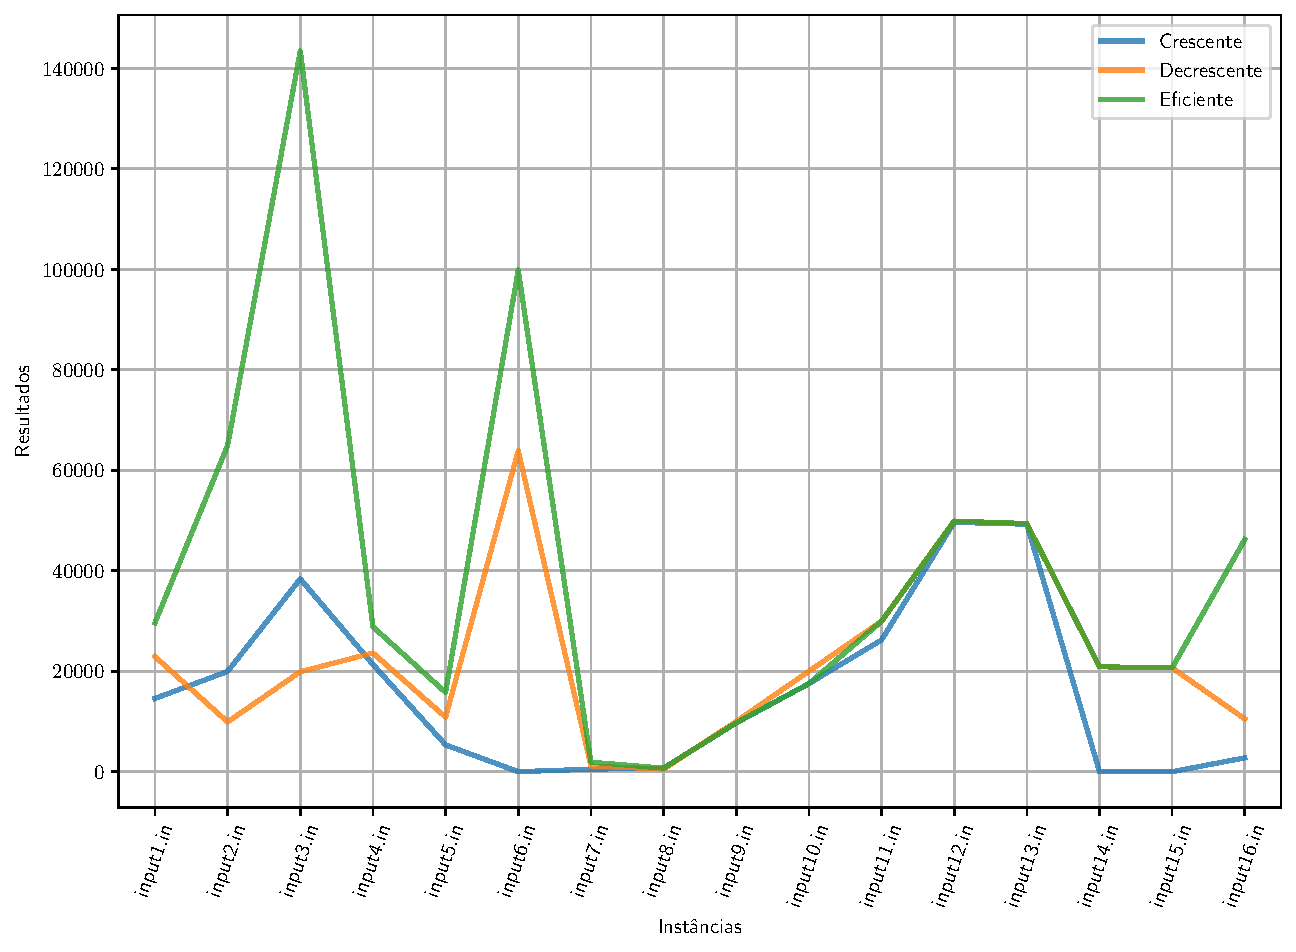
\includegraphics[width=0.7\textwidth]{../imgs/greedy_compare.pdf}
    \caption{\textbf{Figura 1.} Comparação entre resultados das Heurísticas Gulosas.}
    \label{greedy_compare}
\end{figure}

Logo, a seguinte questão é levantada: ''Dentre as Heurísticas Gulosas programadas, qual teria melhor eficiência quando comparado ao resultado de um algoritmo ótimo?''

Como podemos ver na figura abaixo, aparentemente, a Heurística que mais se comparada ao resultado ótimo, é a ''Eficiente''.
\begin{figure}[h]
    \centering
    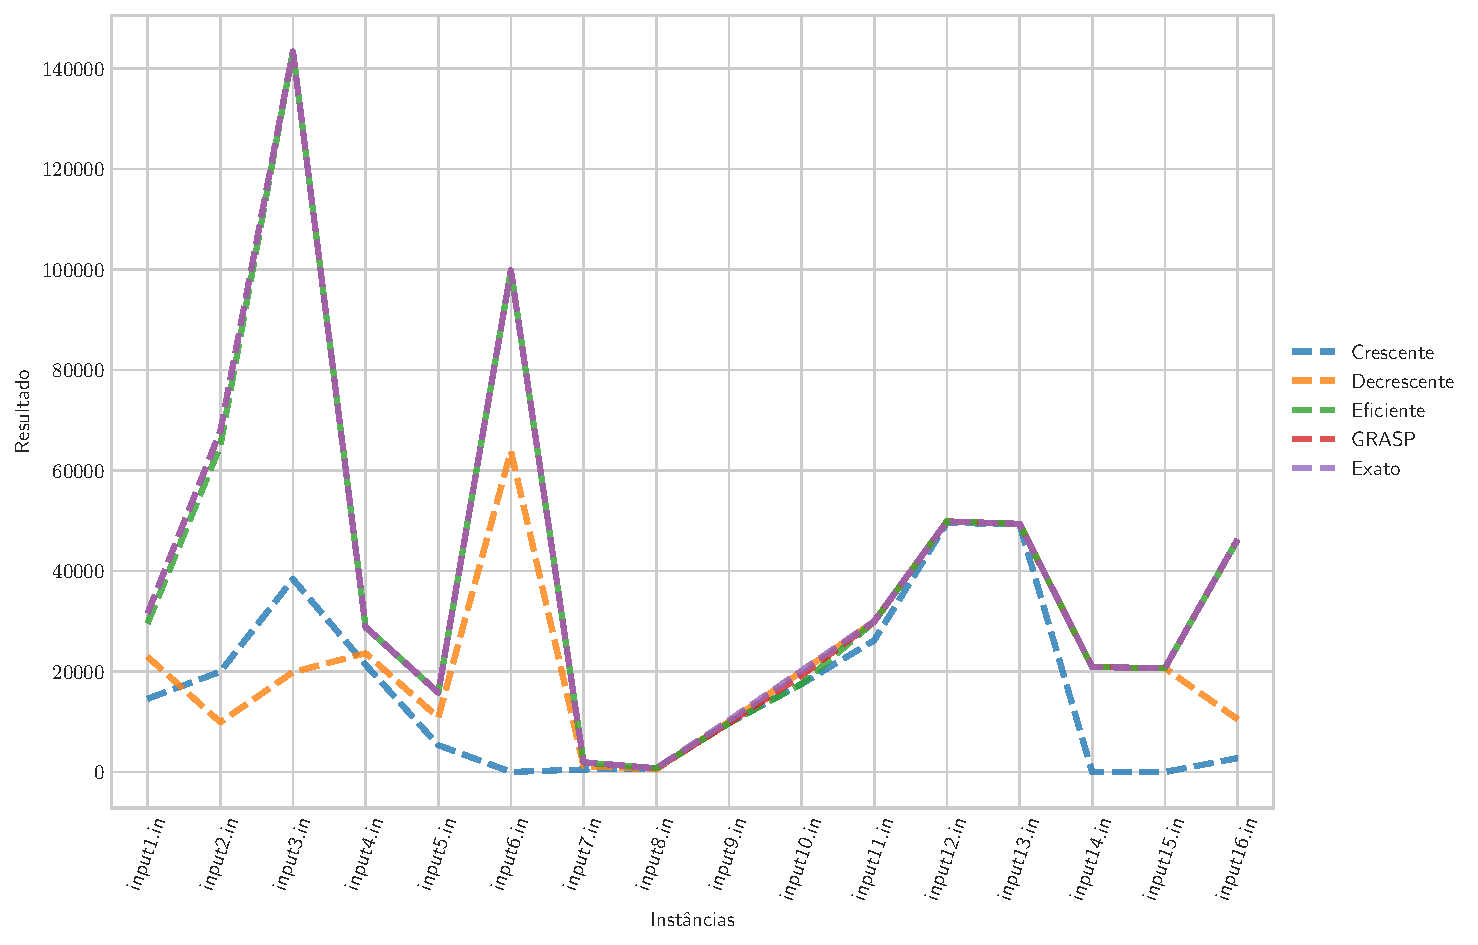
\includegraphics[width=0.7\textwidth]{../imgs/exact_compare.pdf}
    \caption{\textbf{Figura 2.} Comparação entre resultados das Heurísticas Gulosas.}
    \label{exact_compare}
\end{figure}

A fim poder afirmar com mais clareza o resultado do gráfico acima, foi realizado o cálculo da correlação dos valores 
relacionado ao resultado exato.
\begin{figure}[h]
    \centering
    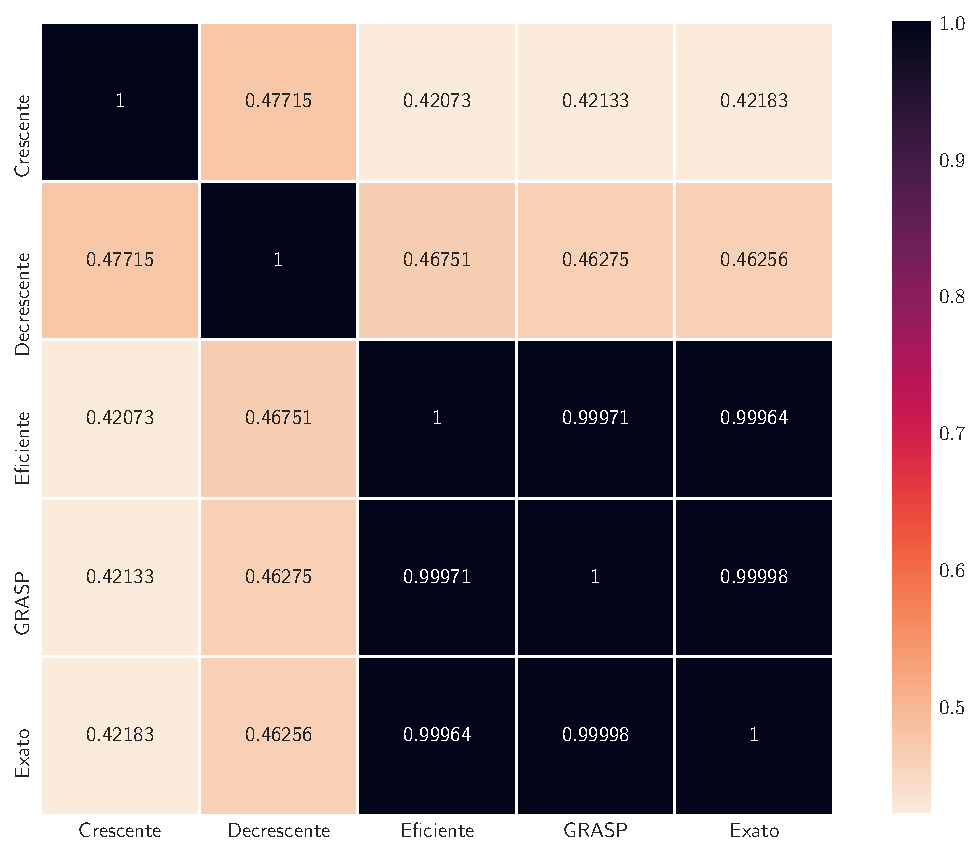
\includegraphics[width=0.7\textwidth]{../imgs/heatmap.pdf}
    \caption{\textbf{Figura 3.} Heatmap para ver a correlação dos resultados obtidos.}
    \label{heatmap}
\end{figure}

Pode se ver que, a correlação \textit{linha/coluna} dos resultados da Heurística ''Eficiente'' quando comparada ao ''Exato'', é de quase $100\%$,
quanto as outras, não chegam a $50\%$.

\section{Interpretação dos Resultados}


\section{Conclusão}

\bibliography{References}{}
\bibliographystyle{plain}

\end{document}